\section{Introduction} \label{section: intro and motiv}

\begin{wrapfigure}{r}{0.45\textwidth}
\vspace{-1.5cm}
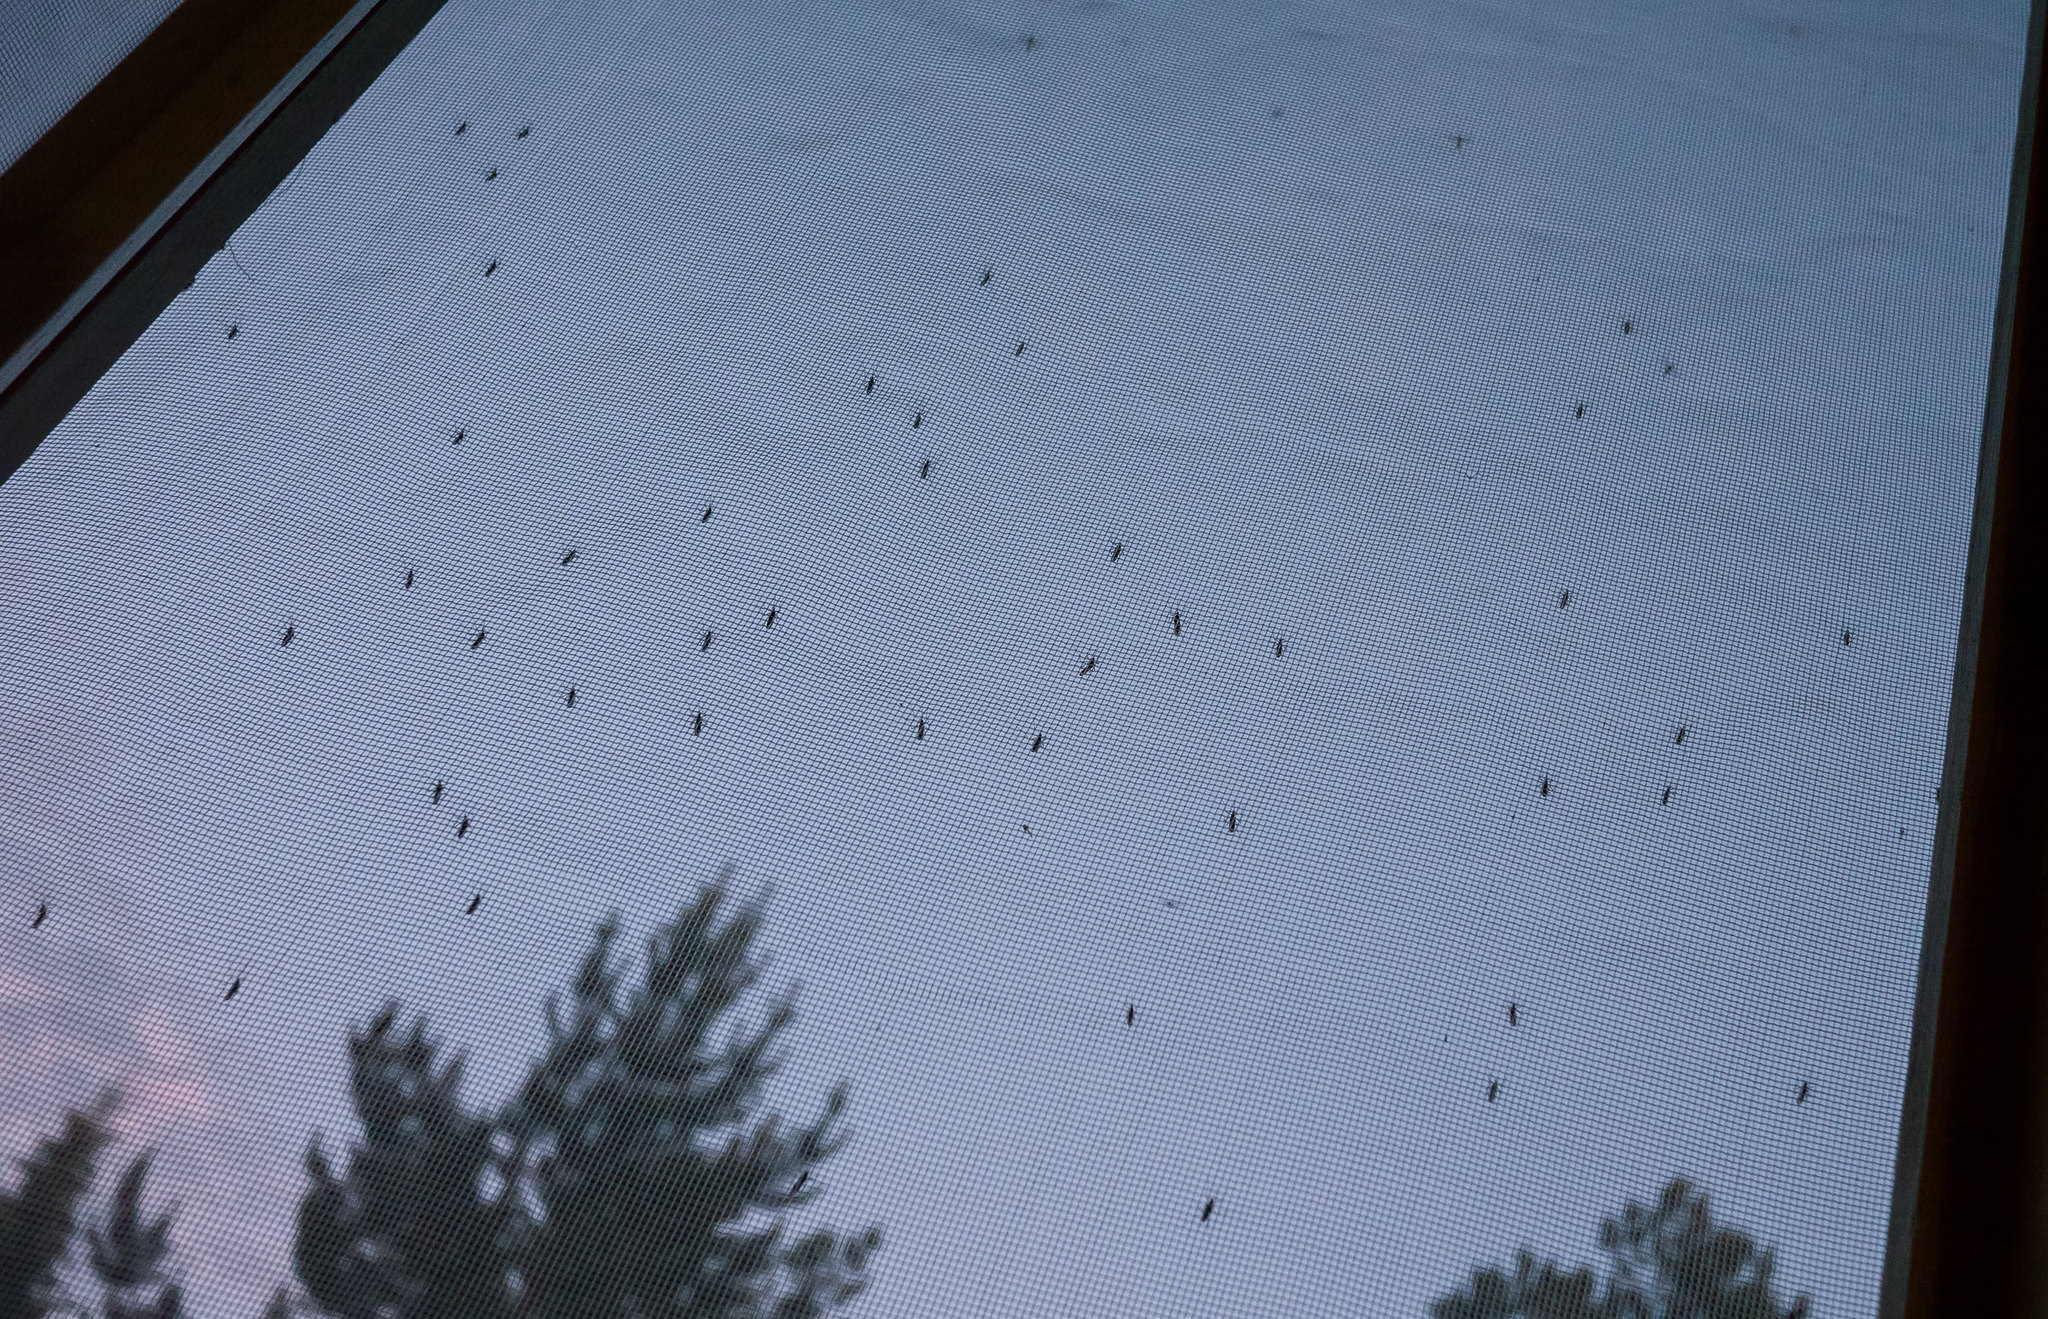
\includegraphics[width=0.9\linewidth]{figures/mosquitogrid.jpg}
\caption{Anti-bug grid (\href{https://www.flickr.com/photos/neekohfi/7817306994/}{Flickr.com})}\
\end{wrapfigure}

Bug grids can be placed over open windows to allow air to flow through without letting bugs into someone's house. Presumably, when people open their windows, they want air to flow through their house. However, the installation of the grid decreases the functional cross-sectional area of the window, which might decrease the airflow. If the properties of the grid cause the flow to become turbulent, the reduction in airflow would be more drastic, than due to the reduction in the cross-sectional area alone. Using a fluid simulation, this report aims to capture this phenomenon, and investigate how the grid's thickness and density affect the airflow through a window. In doing so, an investigation into the optimal parameters of the grid that maximise airflow while "keeping the bugs out" will be conducted. 


\subsection{Research question}
\textbf{Main:}
\begin{itemize}
    \item How much does the air flux through a window with a bug grid change with the grid's thickness and density?
\end{itemize}
\textbf{Subquestions:}
\begin{itemize}
    \item What are the optimal parameters of the grid that maximise airflow while keeping the bugs out?
    \item In which section of the window has the airflow decreased the most due to the presence of the bug grid?
\end{itemize}
